\section{Results and Discussion}
\label{sec:results}
\subsection{Baseline Comparison and Research Questions}
Table~\ref{tab:results} compares manual invocation with automatic suggestions.
Condition values are participant-level means and sample standard deviations;
changes are means of within-person differences with 95\% bootstrap confidence
intervals (CIs). Productivity is measured in completed task fraction/hour.
All 33 pairs contribute to the estimates.

\begin{table*}[t]
\caption{Manual Copilot baseline versus automatic suggestions. Condition values are mean $\pm$ sample SD; changes are automatic minus manual, with participant-pair bootstrap 95\% CIs. Completion changes use percentage points (pp).}
\label{tab:results}
\centering
\begin{tabular}{@{}llrrr@{}}
\toprule
Group & Outcome (unit) & Manual baseline & Automatic & Paired change [95\% CI] \\
\midrule
Novice ($n=17$) & Productivity (task fraction/hour) & $0.182\pm0.153$ & $0.472\pm0.262$ & $+0.290\ [ +0.134, +0.456]$ \\
 & Completion (\%; change in pp) & $18.824\pm16.773$ & $51.029\pm25.831$ & $+32.206\ [ +17.059, +48.235]$ \\
 & Session time (minutes) & $60.588\pm4.963$ & $67.235\pm10.426$ & $+6.647\ [ +1.176, +12.941]$ \\
\midrule
Expert ($n=16$) & Productivity (task fraction/hour) & $0.789\pm0.213$ & $0.513\pm0.338$ & $-0.276\ [ -0.495, -0.049]$ \\
 & Completion (\%; change in pp) & $78.750\pm15.055$ & $55.781\pm30.079$ & $-22.969\ [ -41.098, -4.531]$ \\
 & Session time (minutes) & $61.750\pm11.000$ & $69.438\pm12.296$ & $+7.688\ [ +1.000, +14.625]$ \\
\bottomrule
\end{tabular}
\end{table*}

\textbf{RQ1---Novices:} Mean productivity increased from 0.182 under manual
invocation to 0.472 under automatic suggestions. The mean paired change was
$+0.2901$ task fraction/hour (95\% CI $[+0.1338,+0.4560]$). In this sample,
automatic suggestions were associated with higher novice productivity.
The median paired change was $+0.250$, and the middle half of changes ranged
from $+0.008$ to $+0.375$. These descriptive values indicate variation around
the group mean rather than a uniform improvement for every participant.

\textbf{RQ2---Experts:} Mean productivity decreased from 0.789 to 0.513.
The paired change was $-0.2759$ task fraction/hour (95\% CI
$[-0.4954,-0.0489]$). Manual invocation was associated with higher expert
productivity on average. The median change was $-0.318$, with the middle half
between $-0.594$ and $+0.013$. Thus, the negative mean also coexists with
individual variation. Sample SDs in Table~\ref{tab:results} describe variability
among observations; the CIs describe uncertainty in estimated mean changes.

\textbf{RQ3---Direct group contrast:} The expert-minus-novice difference in
mean paired changes was $-0.5660$ task fraction/hour (95\% CI
$[-0.8387,-0.2839]$). Figure~\ref{fig:changes} displays this contrast alongside
the two group changes. Its interval lies below zero, supporting a lower
mode-related change among experts under the participant-pair resampling
procedure. This answers RQ3 by estimating the difference itself, rather than
comparing separate within-group significance decisions.

\begin{figure}[t]
\centering
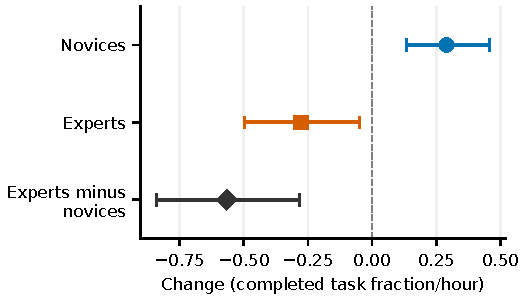
\includegraphics[width=\columnwidth]{figures/fig1_paired_changes.pdf}
\caption{Mean productivity changes and their direct contrast. Horizontal bars
are 95\% participant-pair bootstrap CIs. The dashed line marks zero. The bottom
estimate subtracts the novice change from the expert change.}
\label{fig:changes}
\end{figure}

Absolute productivity and mode-related change answer different questions.
Experts' automatic-mode mean, 0.513, remained slightly above the novice mean,
0.472, although experts had a negative paired change. The larger positive
novice change therefore does not imply that novices outperformed experts in
the automatic condition. Likewise, $-0.5660$ is a difference in task
fraction/hour, not a percentage decline.

\subsection{Completion and Session Time}
Figure~\ref{fig:components} separates the two components of productivity.
Novice mean completion increased from 18.824\% to 51.029\%, a paired increase
of 32.206 pp (95\% CI $[17.059,48.235]$). Mean session time also increased,
by 6.647 minutes (95\% CI $[1.176,12.941]$). The productivity increase thus
accompanied substantially more completed work and longer sessions. It should
be described as higher completed work per hour, rather than faster completion.
The productivity means average individual ratios; they are not ratios of the
group mean completion and group mean time.

\begin{figure}[t]
\centering
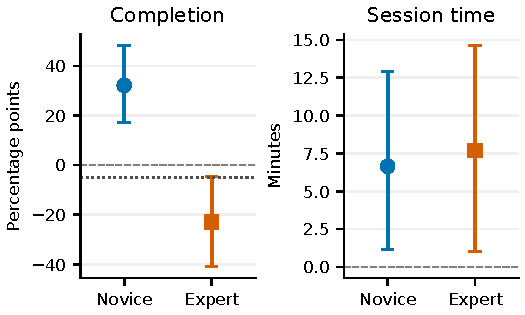
\includegraphics[width=\columnwidth]{figures/fig3_completion_time.pdf}
\caption{Mean automatic-minus-manual changes in completion and session time.
Bars show 95\% participant-pair bootstrap CIs. The dotted completion line marks
the project's $-5$ pp reporting threshold.}
\label{fig:components}
\end{figure}

For experts, mean completion fell from 78.750\% to 55.781\%, a change of
$-22.969$ pp (95\% CI $[-41.098,-4.531]$). Session time increased by 7.688
minutes (95\% CI $[1.000,14.625]$). Lower completion and longer sessions
accompanied the lower productivity estimate. The expert completion drop
crossed the project-defined five-pp reporting threshold; the novice change
did not. This flag highlights an outcome that would be hidden by reporting
productivity alone. It concerns implemented task requirements, not a measured
security score or a comprehensive code-quality assessment.

\subsection{Robustness to Participants and Task Allocation}
Removing each participant in turn produced 33 primary-contrast estimates,
ranging from $-0.6233$ to $-0.5200$ task fraction/hour. Every estimate remained
negative. No single participant removal reversed the direction of the main
comparison. This is a sensitivity range, not a confidence interval: it describes
the effect of these specific omissions rather than sampling uncertainty.

Task-allocation strata revealed further variation. For novices, mean paired
changes were $+0.1098$ when automatic suggestions accompanied task A
($n=9$) and $+0.4929$ when they accompanied task B ($n=8$). Corresponding
expert changes were $-0.6132$ and $+0.0614$ ($n=8$ in each stratum).
These contrasts compare task/mode allocations: each person's manual session
uses the other task. They are not isolated estimates of an automatic-mode
effect on a single task.

Equal weighting of the A/B strata yielded a novice change of $+0.3013$ and
an expert change of $-0.2759$. The resulting group contrast was $-0.5773$,
close to the unadjusted $-0.5660$. Equal weighting leaves the expert estimate
unchanged because its strata have equal sample sizes. The direction of the
overall result therefore persists under this allocation check, even though
the stratum estimates show that task context matters. This calculation
standardizes allocation; it does not adjust for session order or carryover.

\subsection{Interpretation and Research Contribution}
The results extend the source study~\cite{guglielmi2026copilot} with a direct,
reproducible estimate of the between-group difference in paired changes.
They complement interaction accounts distinguishing exploration from
acceleration~\cite{barke2023grounded} and research on uneven benefits for
novices~\cite{prather2024widening}. Our measurements do not distinguish these
interaction mechanisms. For example, interruptions or additional checking
could help explain an expert's lower productivity, but the released
completion/time tables do not test that explanation.

The practical implication is to evaluate suggestion delivery together with
experience and task context. A productivity ratio alone conceals whether a
mode accompanies more completed work, less time, or both. Reporting the
components and the direct contrast makes those distinctions visible.
The contribution is estimation and transparent reconstruction from released
measurements, rather than a new Copilot intervention. Related work supplies
context; the numerical baseline remains manual Copilot invocation in the
same participant sample.
